\documentclass[letterpaper]{article}

\usepackage[utf8]{inputenc}
\usepackage{microtype}
\usepackage[usenames,dvipsnames,svgnames]{xcolor}
\usepackage{menukeys}

\usepackage{listings}
\lstset{
    basicstyle=\scriptsize\ttfamily,
    commentstyle=\color{Gray},
    extendedchars=true,              % lets you use non-ASCII characters; for 8-bits encodings only, does not work with UTF-8
    frame=single,                    % adds a frame around the code
    keepspaces=true,                 % keeps spaces in text, useful for keeping indentation of code (possibly needs columns=flexible)
    keywordstyle=\color{BurntOrange},
    language=C++,
    otherkeywords={void, Servo},
    numbers=left,
    numbersep=5pt,
    numberstyle=\scriptsize,
    rulecolor=\color{black},
    showspaces=false,
    showstringspaces=false,
    showtabs=false,
    stringstyle=\color{Blue},
    tabsize=2
}

\usepackage{graphicx}
\graphicspath{ {img/} }

\title{Build Your First Robot with Arduino}
\author{UW Tacoma IEEE Student Branch}

\begin{document}

\maketitle

An Arduino is an open-source physical computing platform.
That means its a way to program \emph{things}.
You can use an Arduino to control lights, motors, buttons, or almost anything.
Arduinos provide a beginner friendly way to program microcontrollers.
We'll be using the Arduino Uno,
the most standard Arduino model.

\begin{figure}[h!]
    \center
    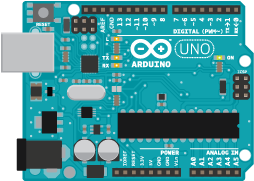
\includegraphics[width=.5\textwidth]{uno.png}
    \caption{Arduino Uno}
\end{figure}

\section{Getting Started}
\label{sec:getting_started}

To program the Arduino,
we'll use the Arduino IDE (integrated development environment).
Open the start menu and type ``arduino'' to find it.
It should look something like Figure~\ref{fig:ide}.

\begin{figure}[h!]
    \center
    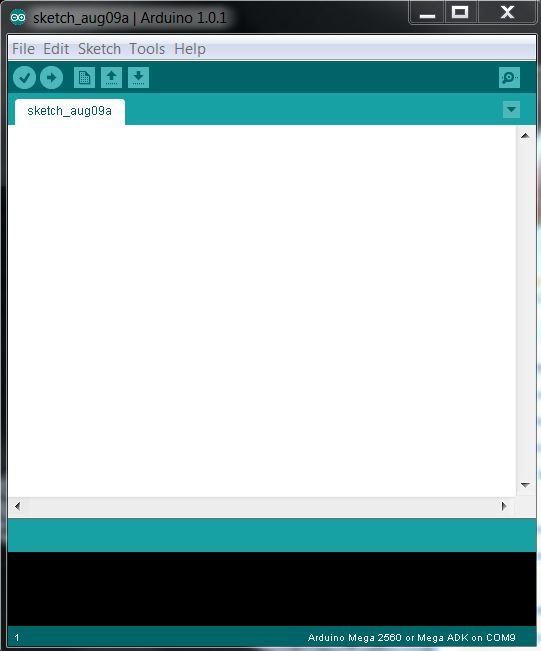
\includegraphics[width=.5\textwidth]{ide.jpg}
    \caption{Arduino IDE}
    \label{fig:ide}
\end{figure}

We'll start by blinking a light with our Arduino.
Select \menu{File>Examples>>01.Basics>Blink}.
This will load the code for a program to blink the light.

Next we put the code onto the board.
Select \menu{Tools>Board>Arduino Uno}.
This tells the program which type of board we're using.
Plug the board into your computer with a USB cable.
Go to \menu{Tools>Port} and make sure something is checked.
This tells the computer where to find your Arduino.
Finally, select \menu{File>Upload}.
A progress bar will show you as the code is sent to the board.

Congratulations!
You have just programmed your Arduino.
You should see the LED (light emitting diode) on your board blinking.

\section{Building Your Robot}
\label{sec:wiring_your_robot}



\clearpage

\lstinputlisting{basic.ino}

\end{document}
